В силу Утверждений 1,2 приходим к

\begin{utv}
Для системы (\ref{fullt}) имеют место:

1.  множества 
$$M_0, M_{0,+}, M_{0,-}, M_{0,b}^{\pm}$$
являются инвариантными.

2. Множество $M_{0,-}$ является также гиперболическим.

3. Пусть $\Big( x(t), y(t), 0, \lambda_{-} \big( x(t),y(t) \big), \Lambda = 0 \Big)$ - некоторая траектория медленной системы (\ref{slowreal}) на $M_{0,-}$, тогда окрестность этой траектории на плоскости $xy$ является инвариантным гиперболическим множеством.

\end{utv}

Найдем явный вид функции Мельникова для исследуемой системы. Для этого приведем уравнения (\ref{fullt}) к виду (\ref{wiggs}):
$$
 X = \begin{pmatrix}
  \Lambda\\
  z
 \end{pmatrix},
 I = \begin{pmatrix}
  x\\
  y
 \end{pmatrix}.$$

Переменная $z$ вводится как:
$$z = \lambda - \lambda_{-}(x,y).$$ 
При этом многообразие $M_{0,-}$ переходит в $\tilde M_{0,-}$:
$$\tilde M_{0,-} = \left\{ (\Lambda, z, x, y): \Lambda = 0,\,\, z=0 \right\},$$
а сепаратриса записывается в виде:
$$z_{sep}(t,t_0) = \pm 2 \arctan{\sh \big( \alpha \beta (t-t_0) \big)}, \Lambda_{sep}(t,t_0) = 2\beta/ \ch \big(\alpha \beta (t-t_0) \big).$$

Тогда в терминах новых переменных имеем:
$$
 D_X = \begin{pmatrix}
  \frac{\partial}{\partial \Lambda}\\
  \frac{\partial}{\partial z}
 \end{pmatrix},
 D_I = \begin{pmatrix}
  \frac{\partial}{\partial x}\\
  \frac{\partial}{\partial y}
 \end{pmatrix},
 $$

$$H_1 = \alpha \frac{\Lambda^2}{2}+\beta(x,y)(1-\cos z),\quad \beta(x,y) = \sqrt{u(x,y)^2+v(x,y)^2},$$

$$g^I = \begin{pmatrix}
  -2Fy+\frac{\partial \beta}{\partial y} \cos z + \beta(x,y) \frac{\partial}{\partial y} \arctan(\frac{v}{u}) \sin z\\
  2Fx +e_JG -\frac{\partial \beta}{\partial x} \cos z - \beta(x,y) \frac{\partial}{\partial x} \arctan(\frac{v}{u}) \sin z
 \end{pmatrix},$$

$$g^X = \frac{-1}{\varepsilon} \begin{pmatrix}
  0 \\
  \frac d{dt} \arctan(\frac vu)
 \end{pmatrix}
 = 
 \frac{-(u \dot v - v \dot u)}{\varepsilon \beta^2} \begin{pmatrix}
  0 \\
  1
 \end{pmatrix}
 =
 \frac{-\Big(\dot x \big(u \frac{\partial v}{\partial x} - v \frac{\partial u}{\partial x} \big) + \dot y \big(u \frac{\partial v}{\partial y} - v \frac{\partial u}{\partial y}\big) \Big)}{\varepsilon \beta^2} \begin{pmatrix}
  0 \\
  1
 \end{pmatrix} = 
 $$
 
$$
 =
 \frac{\big(2Fy+\frac{\partial u}{\partial y} \cos \lambda + \frac{\partial v}{\partial y} \sin \lambda \big) \big(u \frac{\partial v}{\partial x} - v \frac{\partial u}{\partial x}\big) - \big(2Fx+e_JG +\frac{\partial u}{\partial x} \cos \lambda + \frac{\partial v}{\partial x} \sin \lambda \big) \big(u \frac{\partial v}{\partial y} - v \frac{\partial u}{\partial y} \big)}{\beta^2} \begin{pmatrix}
  0 \\
  1
 \end{pmatrix}.
 $$

\subsection{Расщепление сепаратрис}

Построим функцию Мельникова для множества $V=\tilde M_{0,-}$ из Теоремы 5.
Для этого сначала отдельно посчитаем подинтегральное выражение:
$$<D_IH_1, g^I> = (1 - \cos z) \Bigg( -2Fy \frac{\partial \beta}{\partial x}+(2Fx+e_J G)\frac{\partial \beta}{\partial y} + \frac{\sin z}{\beta} \bigg( 
\frac{\partial \beta}{\partial y}\Big(v \frac{\partial u}{\partial y}-u \frac{\partial v}{\partial y}\Big)-\frac{\partial \beta}{\partial x}\Big(v \frac{\partial u}{\partial x}-u \frac{\partial v}{\partial x} \Big)   \bigg)    \Bigg),$$

$$<D_XH_1,g^X> = \frac{- \beta  \sin z}{\varepsilon} \frac{d}{dt}{\Big( \arctan \frac{v}{u} \Big)},$$

$$D_I H_1 \big( v(I),I \big) = \begin{pmatrix}
  0 \\
  0
\end{pmatrix}.
$$

Тогда:
$$M^I(x,y) = \int_{-\infty}^{\infty}\big(1-\cos z_{sep}(t)\big)dt \bigg( -2Fy \frac{\partial \beta}{\partial x} + (2Fx+e_J G) \frac{\partial \beta}{\partial y} \bigg) + $$
$$+ \frac{1}{\beta} \int_{-\infty}^{\infty} \sin z_{sep}(t)dt \Bigg( 
\bigg(v \frac{\partial u}{\partial y}-u \frac{\partial v}{\partial y}\bigg) \Big(-\frac{\partial \beta}{\partial x} + 2Fx+e_JG \Big)+\bigg(v \frac{\partial u}{\partial x}-u \frac{\partial v}{\partial x}\bigg) \Big(\frac{\partial \beta}{\partial y} - 2Fy \Big)
\Bigg).$$
Подставляя выражение для $z_{sep}$, получаем:
$$\int_{-\infty}^{\infty} \big(1-\cos z_{sep}(t) \big)dt = \int_{-\infty}^{\infty}\frac{2}{\ch^{2}(\alpha\beta t)}dt = \frac{4}{\alpha \beta},$$
$$\int_{-\infty}^{\infty} \sin z_{sep}(t)dt = \int_{-\infty}^{\infty}\frac{2\sh(\alpha\beta t)}{\ch^{2}(\alpha\beta t)}dt = 0.$$
Следовательно,
$$M^I(x,y)= \frac{4}{\alpha \beta} \left( 
    -2Fy \frac{\partial \beta}{\partial x} + (2Fx+e_J G) \frac{\partial \beta}{\partial y}
\right) = $$
$$ = \frac{4}{\alpha \beta^2} \Bigg( 
    u \bigg( (2Fx+e_J G)\frac{\partial u}{\partial y} - 2Fy \frac{\partial u}{\partial x} \bigg) + 
    v \bigg((2Fx+e_J G)\frac{\partial v}{\partial y} - 2Fy \frac{\partial v}{\partial x} \bigg)
\Bigg) = $$
$$ = \frac{4 Cy}{\alpha \beta^2} \Big( 
    -2u \big( (2Fx+e_J G)+F(2x+\tilde \alpha) \big)+C(2x+\tilde \alpha) \big( (2Fx+e_JG)(2x+\tilde \alpha)-4Fy^2 \big)
\Big).$$

Множество нулей функции Мельникова определяется уравнением:
$$ 0 = y \left( 
    (2x+\tilde \alpha)^2+y^2-(2x+\tilde \alpha)\frac{4FK}{C(e_JG-F \tilde \alpha)} - \frac KC
\right),$$
и состоит из прямой $y=0$ и эллипса (см. рис. \ref{zeroes}).

\begin{figure}[H]
\centering
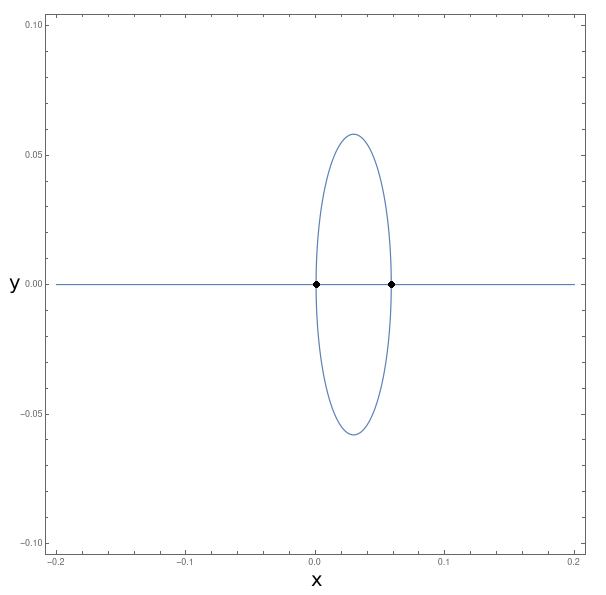
\includegraphics[scale=0.45]{../img/zeros.png}
\caption{Множество нулей функции Мельникова. Черным обозначены нули ее градиента}
\label{zeroes}
\end{figure}

Градиент функции Мельникова $D_IM^I$ обращается в ноль в двух точках на этом множестве:
$$y_M = 0,$$
$$x_M = \frac{-\tilde \alpha}{2}+\frac{FK}{C(e_JG-F \tilde \alpha)} \pm \sqrt{\frac{F^2 K^2}{C^2(e_JG-F \tilde \alpha)}+\frac{K}{4C}}.$$

Таким образом, имеет место следующее
\begin{utv}


1. Пусть $\{\Big( x(\tau), y(\tau), 0, \lambda_{-} \big(x(\tau), y(\tau) \big) \Big), \tau\in \mathbb{R}\} \in M_{0,-}$ - орбита медленной системы (\ref{slowreal}) на листе $M_{0,-}$, 
а $D_0$ -  $\delta$-окрестность этой орбиты в $M_{0,-}$, не содержащая особых точек $(x_{b}^{\pm}, y_{b})$. Тогда для любого достаточно малого $\varepsilon > 0$ существуют локально инвариантное гиперболическое множество $D_\varepsilon$ системы (\ref{fullt}), устойчивое и неустойчивое локально инвариантные многообразия которого пересекаются трансверсально.

2. Для всех $\varepsilon>0$ точка $\big( x_{0}^{-}, y_{0}^{-}, 0, \lambda_{-}(x_{0}^{-}, y_{0}^{-}) \big)$ является гиперболическим положением равновесия системы (\ref{slowreal}).
При этом, для любого достаточно малого $\varepsilon > 0$ устойчивое и неустойчивое инвариантные многообразия, отвечающие этому положению равновесия, пересекаются трансверсально.
\end{utv}
\textbf{Доказательство:}

Множество $D_0$ является компактным инвариантным гиперболическим подмножеством $M_{0,-}$. Тогда по теореме Феничеля для любого достаточно малого $\varepsilon > 0$ существует локально инвариантное множество $D_\varepsilon$, лежащее в $\varepsilon$ окрестности $D_0$. В силу того, что орбита медленной системы имеет непустое пересечение с множеством нулей функции Мельникова, доказываем первое утверждение.

Далее заметим, что точка
$$\big(x_{0}^{-}, y_{0}^{-}, 0, \lambda_{-}(x_{0}^{-}, y_{0}^{-}) \big)$$
является неподвижной гиперболической точкой и для медленной системы (\ref{slow_sys}), и для полной системы (\ref{fullt}). Поэтому при возмущении она остается неподвижной и, следовательно, глобально инвариантным гиперболическим множеством полной системы.

Взяв декартово произведение сепаратрисы быстрой системы и сепаратрисы медленной системы в качестве нулевого приближения для устойчивого и неустойчивого инвариантных многообразий полной системы, а также учитывая то, что сепаратриса медленной системы пересекается с множеством нулей функции Мельникова (см. рис. \ref{sep_zero}), получаем второе утверждение. 

\begin{figure}[H]
\centering
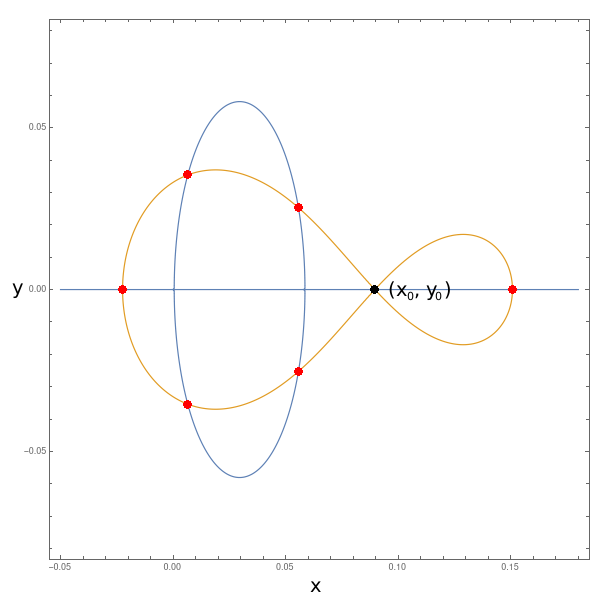
\includegraphics[scale=0.45]{../img/melnikov-separatrix.png}
\caption{Пересечение медленной сепаратрисы на неустойчивом листе $M_{0,-}$ и множества нулей функции Мельникова}
\label{sep_zero}
\end{figure}
%%%%%%%%%%%%%%%%%%%%%%%%%%%%%%%%%%%%%%%%%%%%%%%%%%%%%%%%%%%%%%%%%%%